\chapter{Preliminares}

\section{Teoría de Lenguajes}

En esta sección se definirán los principales conceptos de teoría de lenguajes que sirven de base al contenido de las secciones posteriores.

\subsection{Conceptos básicos}

\paragraph{Alfabeto:} Un alfabeto, denotado como $\Sigma$, es un conjunto finito y no vacío de símbolos, ejemplo:
$$\Sigma=\{1,0\}$$
\paragraph{Cadena:} Una cadena es una sucesión finita de símbolos del alfabeto, ejemplo: la representación binaria de
los números $3=11$ y $5=101$ puede ser un ejemplo de cadena sobre el alfabeto $\Sigma$ anteriormente
definido.
\paragraph{Lenguaje:} Un lenguaje es un conjunto de cadenas definido sobre un alfabeto, ejemplo: el lenguaje de la
representación binaria de todos los números pares $L=\{w\,|\,\text{last}(w)=0\}$, $\text{last}(w)$
representa el último caracter de la cadena $w$.

Dados los conceptos básicos, ahora es necesario definir las operaciones básicas entre los elementos de la teoría de lenguajes.

\subsection{Operaciones con Lenguajes}

Las principales operaciones con lenguajes tienen su origen en la teoría de conjuntos ya que un lenguaje no es más que
un conjunto de cadenas.

\paragraph{Unión:} La unión de dos lenguajes $L_1$ y $L_2$ se define como el conjunto de cadenas que
pertenecen a $L_1$ o a $L_2$:
$$L_1\cup L_2=\{w\,|\,w\in L_1\,\vee\,w\in L_2\}$$
\paragraph{Intersección:} La intersección de dos lenguajes $L_1$ y $L_2$ se define como el conjunto de
cadenas que pertenecen a $L_1$ y a $L_2$:
$$L_1\cap L_2=\{w\,|\,w\in L_1\,\wedge\,w\in L_2\}$$
\paragraph{Concatenación:} La concatenación de dos lenguajes $L_1$ y $L_2$ se define como el conjunto
de cadenas que resultan de concatenar una cadena de $L_1$ con una cadena de $L_2$:
$$L_1\circ L_2=\{w_1w_2\,|\,w_1\in L_1\,\wedge\,w_2\in L_2\}$$
\paragraph{Complemento:} El complemento de un lenguaje $L$ se define como el conjunto de cadenas que no
pertenecen a $L$:
$$\overline{L}=\{w\,|\,w\notin L\}$$
\paragraph{Clausura de Kleene:} La clausura de Kleene de un lenguaje $L$ se define como el conjunto de
cadenas que resultan de concatenar cero o más cadenas de $L$:
$$L^*=\{w_1w_2\ldots w_n\,|\,n\geq 0\,\text{y}\,w_i\in L\}$$

Todos los conceptos anteriormente planteados definen la base de la teoría de lenguajes y de estos se derivan algunas 
preguntas como la siguiente: ¿es posible determinar si una cadena pertenece a un lenguaje?

\subsection{Problemas relacionados con Lenguajes}

Los problemas relacionados con la teoría de lenguajes permiten vincular los problemas de otra naturaleza 
con su representación en la teoría de lenguajes formales. Por ejemplo como puedo determinar si un lápiz 
pertenece al conjunto de los lápices negros.

\paragraph{Problema de la palabra:} Consiste en determinar si una cadena pertenece a un lenguaje dado. Todo problema en Ciencias de la Computación puede ser reducido a un problema de la palabra, ya que cualquier problema
puede ser codificado como un lenguaje formal.
\paragraph{Problema del vacío:} Consiste en determinar si un lenguaje es vacío. Ejemplo se define el lenguaje de la
representación binaria de todos los números pares tales que su último símbolo es 1, $L=\{w\,|\,\text{last}(w)=1 \wedge \text{is\_even(w)}\}$, $\text{last}(w)$ y $\text{is\_even}(w)$
determinan el último símbolo del número y si el número es par o no, respectivamente.
\paragraph{Problema de la finitud:} Consiste en determinar si un lenguaje es finito. Ejemplo se define el lenguaje de todos los números primos en su representación binaria
$L=\{w\,|\,w\in \{0,1\}^+ \wedge \text{is\_prime}(w) \}$, $\text{is\_prime}(w)$ determina si el número que representa $w$ es primo, el problema de la finitud sobre $L$ sería 
determinar si el Conjunto de cadenas el finito o no.
\paragraph{Problema de la equivalencia:} Consiste en determinar si dos $L_1$ y $L_2$ lenguajes son iguales (es decir si se cumple que
$L_1\subseteq L_2 \wedge L_2\subseteq L_1$).

En la próxima sección se presenta una mecanismo formal para definir un lenguaje.

\subsection{Gramáticas}

Una \textbf{gramática} es un formalismo utilizado para describir lenguajes formales. Se define como una 4-tupla:
\[
      G = (N, \Sigma, P, S),
\]
donde:
\begin{itemize}
      \item \(N\): Es un conjunto finito de \textbf{símbolos no terminales}, que representan variables o categorías intermedias.
      \item \(\Sigma\): Es un conjunto finito de \textbf{símbolos terminales}, que constituyen el alfabeto del lenguaje. Se cumple que \(N \cap \Sigma = \emptyset\).
      \item \(P\): Es un conjunto finito de \textbf{reglas de producción}, cada una de la forma:
            \[
                  \alpha \to \beta, \quad \text{donde } \alpha \in (N \cup \Sigma)^* \wedge \beta \in (N \cup \Sigma)^*.
            \]
      \item \(S\): Es el \textbf{símbolo inicial}, \(S \in N\), que define el punto de partida para derivar cadenas del lenguaje.
\end{itemize}

Una derivación en la gramática consiste en seleccionar una \textbf{regla de producción} $\alpha \to \beta$ y sustituir una ocurrencia de 
$\alpha$ en una cadena $w$ por $\beta$.

Una cadena $w$, $w\in\Sigma^*$,  es reconocida por la gramática si existe una secuencia de derivaciones que comienza con $S$ y termina generando la cadena $w$.

El lenguaje generado por una gramática \(G\) se denota como:
\[
      L(G) = \{ w \in \Sigma^* \mid S \overset{*}{\to} w \},
\]
donde \(\overset{*}{\to}\) indica una derivación en cero o más pasos.

Ahora es necesario conocer la relación de la estructura de las reglas de producción de una gramática con su poder 
para describir lenguajes.

\subsection{Jerarquía de Chomsky}

La \textbf{Jerarquía de Chomsky} (Figura~\ref{fig:ChomskySchema}) clasifica las gramáticas en cuatro tipos, según las restricciones en sus reglas de producción y la capacidad expresiva de los lenguajes que generan.

\begin{enumerate}
      \item \textbf{Tipo 0: Gramáticas irrestrictas}
            \begin{itemize}
                  \item No tienen restricciones en las reglas de producción.
                  \item Cada regla tiene la forma: \(\alpha \to \beta\), donde \(\alpha, \beta \in (N \cup \Sigma)^*\) y \(\alpha \neq \varepsilon\).
                  \item Todo lenguaje generado por una gramática irrestricta se denomina \textbf{lenguaje recursivamente enumerable}.
            \end{itemize}
            
      \item \textbf{Tipo 1: Gramáticas dependientes del contexto}
            \begin{itemize}
                  \item Cada regla tiene la forma: \(\alpha A \gamma \to \alpha \beta \gamma\), donde \(A \in N\), \(\alpha, \beta, \gamma \in (N \cup \Sigma)^*\), y \(|\beta| \geq 1\).
                  \item Todo lenguaje generado por una gramática dependiente del contexto se denomina \textbf{lenguaje dependiente del contexto}.
            \end{itemize}
            
      \item \textbf{Tipo 2: Gramáticas libres del contexto}
            \begin{itemize}
                  \item Cada regla tiene la forma: \(A \to \beta\), donde \(A \in N\) y \(\beta \in (N \cup \Sigma)^*\).
                  \item Todo lenguaje generado por una gramática libre del contexto se denomina \textbf{lenguaje libre del contexto}.
            \end{itemize}
            
      \item \textbf{Tipo 3: Gramáticas regulares}
            \begin{itemize}
                  \item Las reglas tienen la forma:
                        \[
                              A \to aB \quad \text{o} \quad A \to a,
                        \]
                        donde \(A, B \in N\) y \(a \in \Sigma\).
                  \item Todo lenguaje generado por una gramática regular se denomina \textbf{lenguaje regular}.
            \end{itemize}
\end{enumerate}


\begin{figure}
      \centering
      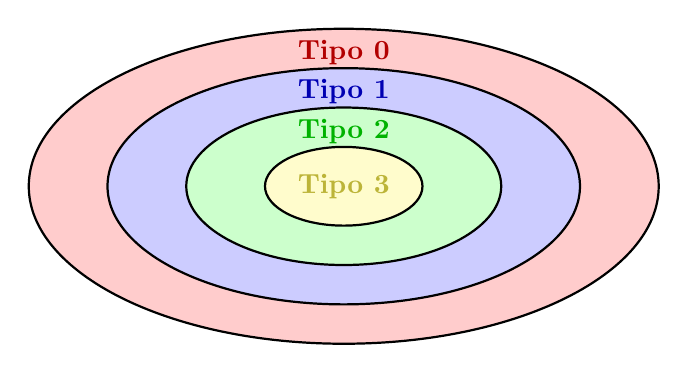
\begin{tikzpicture}[scale=1]
            \draw[thick, fill=red!20] (0,0) ellipse (4cm and 2cm);
            \node at (0,1.7) {\textbf{\textcolor{red!70!black}{Tipo 0}}};
            
            \draw[thick, fill=blue!20] (0,0) ellipse (3cm and 1.5cm);
            \node at (0,1.2) {\textbf{\textcolor{blue!70!black}{Tipo 1}}};
            
            \draw[thick, fill=green!20] (0,0) ellipse (2cm and 1cm);
            \node at (0,0.7) {\textbf{\textcolor{green!70!black}{Tipo 2}}};
            
            \draw[thick, fill=yellow!20] (0,0) ellipse (1cm and 0.5cm);
            \node at (0,0) {\textbf{\textcolor{yellow!70!black}{Tipo 3}}};
      \end{tikzpicture}
      \caption{Esquema de la Jerarquía de Chomsky}
      \label{fig:ChomskySchema} %
\end{figure}

En la próxima sección se presentan los principales conceptos relacionados con las gramáticas libres del contexto y las 
gramáticas regulares.

\section{Autómatas}
Un autómata es el modelo de cómputo más básico en la teoría de lenguajes, pero estos son capaces de describir
una gran variedad de lenguajes. En esta sección se abordarán los principales conceptos sobre los autómatas.
\subsection{Autómata regular}

Un autómata regular \cite{authomataTheory}, también conocido como autómata finito, es un modelo matemático para reconocer lenguajes regulares. Este tipo de autómata se define como una máquina abstracta que procesa cadenas de símbolos de un alfabeto finito y determina si una cadena pertenece a un lenguaje regular.

Un autómata regular se puede representar como una 5-tupla $$\mathcal{A} = (Q, \Sigma, \delta, q_0, F),$$ donde:

\begin{itemize}
      \item $Q$: Es un conjunto finito de \textbf{estados}.
      \item $\Sigma$: Es el \textbf{alfabeto} finito de entrada.
      \item $\delta$: Es la \textbf{función de transición}, $\delta: Q \times \Sigma \to Q$, que define cómo el autómata cambia de estado en función del símbolo leído.
      \item $q_0 \in Q$: Es el \textbf{estado inicial} desde donde comienza la computación.
      \item $F \subseteq Q$: Es el conjunto de \textbf{estados de aceptación o estados finales}.
\end{itemize}

El autómata comienza en el estado inicial $q_0$ y procesa una cadena de entrada símbolo por símbolo. En cada paso, la función de transición $\delta$ determina el siguiente estado del autómata. Si, después de procesar toda la cadena, el autómata termina en un estado de aceptación $q \in F$, entonces la cadena es aceptada; de lo contrario, es rechazada.

Se puede extender el concepto de autómata finito añadiendo un nuevo tipo de transición que no consume ningún caracter, la cual recibe el nombre de transición $\varepsilon$.
Se puede demostrar que el conjunto de lenguajes reconocido por un autómata finito sin transiciones $\varepsilon$ (\textit{autómata finito determinista}) es equivalente al conjunto de lenguajes reconocidos por un autómata finito con transiciones $\varepsilon$ (\textit{autómata finito no determinista}).

\subsection{Autómata de pila y Gramáticas libres del contexto}

Un autómata de pila \cite{authomataTheory} es un modelo matemático de computación que extiende los autómatas finitos al incluir una estructura de datos adicional: una pila. Este modelo es capaz de reconocer lenguajes libres de contexto,
proporcionando una conexión directa con las gramáticas libres de contexto \textit{CFG}, es decir dada una gramática libre del contexto se puede construir un autómata de pila que reconozca el lenguaje generado por la gramática y viceversa.

Formalmente, un autómata de pila se define como una 7-tupla
\[
      \mathcal{A} = (Q, \Sigma, \Gamma, \delta, q_0, Z_0, F),
\]
donde:

\begin{itemize}
      \item $Q$: Es un conjunto finito de \textbf{estados}.
      \item $\Sigma$: Es el \textbf{alfabeto} finito de entrada.
      \item $\Gamma$: Es el \textbf{alfabeto} finito de la pila (conjunto de símbolos que se pueden almacenar en la pila).
      \item $\delta$: Es la función de transición, $\delta: Q \times (\Sigma \cup \{\varepsilon\}) \times \Gamma \to \mathcal{P}(Q \times \Gamma^*)$, que describe cómo cambia el estado, el contenido de la pila y la posición en la entrada.
      \item $q_0 \in Q$: Es el \textbf{estado inicial} desde donde comienza la computación.
      \item $Z_0 \in \Gamma$: Es el símbolo inicial en la pila.
      \item $F \subseteq Q$: Es el conjunto de \textbf{estados de aceptación o estados finales}.
\end{itemize}

Un autómata de pila procesa una cadena de entrada desde el estado inicial $q_0$ y 
puede utilizar transiciones $\varepsilon$ (sin consumir entrada). En cada paso, la función $\delta$
determina el nuevo estado, los símbolos que se insertan o sacan de la pila, y el avance en la entrada, 
tras procesar toda la cadena, el autómata termina en un estado de aceptación o con una pila vacía 
(dependiendo del criterio de aceptación), la cadena es aceptada.

A continuación se presentan las principales transformaciones entre lenguajes formales.

\section{Transformaciones en Lenguajes Formales}

Una transformación entre lenguajes no es más que una función que define una correspondencia una cadena
de un lenguaje $L_1$ y una cadena de un lenguaje $L_2$.

\subsection{Homorfismo}

Dado un alfabeto \( \Sigma \) y un alfabeto \( \Gamma \), un homomorfismo es una función:
\[
      h: \Sigma^* \to \Gamma^*
\]
tal que:
\begin{enumerate}
      \item Para cada \( a \in \Sigma \), \( h(a) \) es una cadena en \( \Gamma^* \).
      \item Para cualquier par de cadenas \( u, v \in \Sigma^* \), se cumple que:
            \[
                  h(uv) = h(u) h(v),
            \]
            es decir, el homomorfismo preserva la concatenación.
\end{enumerate}

\subsection{Transductor finito}

Un transductor finito es un modelo computacional que extiende los autómatas finitos al incluir tanto entradas como salidas.
Formalmente, un transductor finito es un autómata finito determinista o no determinista con una función de transición extendida
que asocia una salida a cada transición.

Un transductor finito puede representarse como una 6-tupla:
\[
      T = (Q, \Sigma, \Gamma, \delta, q_0, F),
\]
donde:
\begin{itemize}
      \item \(Q\) es el conjunto finito de estados.
      \item \(\Sigma\) es el alfabeto de entrada.
      \item \(\Gamma\) es el alfabeto de salida.
      \item \(\delta: Q \times \Sigma \to Q \times \Gamma^*\) es la función de transición, que mapea una combinación de estado actual y símbolo de entrada a un nuevo estado y una salida.
      \item \(q_0 \in Q\) es el estado inicial.
      \item \(F \subseteq Q\) es el conjunto de estados finales.
\end{itemize}

Observe que un homorfismo es un transductor finito de un solo estado y tantas transiciones hacia el mismo estado como transformaciones
de símbolos en el homomorfismo.

En este punto se conoce la clasificación de las gramáticas según la Jerarquía de Chomsky 
y a su vez la clasificación de los lenguajes que estas generan, puede parecer que existen lenguajes
más difíciles de describir que otros y que a su vez traen consigo problemas más difíciles que otros, 
por lo que se hace necesario definir que tan difícil o que tan sencillo puede resultar un problema en sí 
o comparado con otro. 

\section{Complejidad computacional}

En esta sección se definen los principales conceptos de complejidad computacional y las clases de problemas.

\subsection{Máquina de Turing}

Una Máquina de Turing \cite{authomataTheory} es un modelo abstracto de computación universal introducido por Alan Turing en 1936. Este modelo consiste en los siguientes componentes:

\begin{itemize}
      \item \textbf{Cinta}: Un medio de almacenamiento infinito dividido en celdas, donde cada celda contiene un símbolo de un alfabeto finito.
      \item \textbf{Cabezal de lectura/escritura}: Un dispositivo que puede leer el contenido de una celda, escribir un nuevo símbolo y moverse a la izquierda o derecha.
      \item \textbf{Conjunto de estados}: Una colección finita de estados internos que describen la configuración actual de la máquina.
      \item \textbf{Función de transición}: Un conjunto de reglas que determinan cómo la máquina cambia de estado, escribe en la cinta y mueve el cabezal en función del estado actual y el símbolo leído.
\end{itemize}

\paragraph{Máquina de Turing determinista (\textit{DTM}):}
En una Máquina de Turing determinista, para cada estado y cada símbolo leído, existe como máximo una transición
definida.
\paragraph{Máquina de Turing no determinista (\textit{NTM}):}
En una Máquina de Turing no determinista, para cada estado y símbolo leído, pueden existir múltiples
transiciones posibles.

Una Máquina de Turing define el límite entre lo computable y lo no computable, lo cual es la base para el concepto de 
algoritmo en Ciencias de la Computación.

A continuación se presenta una notación para describir el tiempo que demora un algoritmo en realizar determinado cómputo.

\subsection{Notación asintótica}

La notación asintótica se utiliza para describir el comportamiento de una función $f(n)$ a medida que $n$ crece hacia el infinito. A continuación se definen las notaciones más comunes:

\begin{itemize}
      \item \textbf{Notación $O(f(n))$}: Una función $g(n)$ pertenece a $O(f(n))$ si existen constantes positivas $c$ y $n_0$ tales que:
            \[
                  g(n) \leq c \cdot f(n) \quad \text{para todo } n \geq n_0.
            \]
            Esta notación proporciona un límite superior asintótico para $g(n)$.
            
      \item \textbf{Notación $\Omega(f(n))$}: Una función $g(n)$ pertenece a $\Omega(f(n))$ si existen constantes positivas $c$ y $n_0$ tales que:
            \[
                  g(n) \geq c \cdot f(n) \quad \text{para todo } n \geq n_0.
            \]
            Esta notación proporciona un límite inferior asintótico para $g(n)$.
            
      \item \textbf{Notación $\Theta(f(n))$}: Una función $g(n)$ pertenece a $\Theta(f(n))$ si:
            \[
                  g(n) \in O(f(n)) \quad \text{y} \quad g(n) \in \Omega(f(n)).
            \]
            Es decir, $f(n)$ acota a $g(n)$ tanto superior como inferiormente.
\end{itemize}

La notación asintótica permite describir el tiempo de ejecución un algoritmo en cuanto al número de operaciones básicos realizadas
por un modelo formal de cómputo (por ejemplo una máquina de Turing). Algoritmos como determinar el mínimo y el máximo de
un array son $\Theta(n)$, ya que necesitan realizar una cantidad de operaciones de orden $n$ en relación con el tamaño de la entrada.

En la próxima sección se presenta la clasificación de los problemas de acuerdo a su complejidad computacional.
\subsection{Clases de problemas}

Los problemas computacionales \cite{authomataTheory} se agrupan en diferentes clases según los recursos necesarios para resolverlos.

\paragraph{Problemas en la clase P:}
Un problema pertenece a la clase P si puede resolverse en tiempo polinomial mediante una Máquina de Turing determinista. Es decir, existe un algoritmo determinista que, para una entrada de tamaño $n$, produce la solución en tiempo $O(n^k)$ para alguna constante $k$.

\paragraph{Problemas en la clase NP:}
Un problema pertenece a NP si su solución puede verificarse en tiempo polinomial mediante una Máquina de Turing determinista. Alternativamente, un problema está en NP si puede resolverse en tiempo polinomial mediante una Máquina de Turing no determinista.

\paragraph{Problemas en la clase NP-Completo:}
Un problema pertenece a la clase NP-Completo, si pertenece a NP y además es tan difícil como cualquier otro problema en NP. Esto significa que cualquier problema en NP puede reducirse a este problema en tiempo polinómico.

\paragraph{Problemas no decidibles:}
Un problema es no decidible si no existe una Máquina de Turing que pueda resolverlo correctamente para todas las entradas posibles. Esto significa que no hay algoritmo que garantice una respuesta en tiempo finito en todos los casos. Un ejemplo clásico de problema no decidible es el \textit{Problema de la Parada} \cite{authomataTheory},
que consiste en determinar si una Máquina de Turing se detendrá para una entrada dada.

En este punto se puede formular la siguiente pregunta: ¿realmente existen problemas más difíciles que otros?
\subsection{P vs NP}

La relación entre las clases P y NP es uno de los problemas abiertos más importantes en la teoría de la
computación \cite{authomataTheory}. Hasta la fecha, se desconoce si $\text{P} = \text{NP}$ o si $\text{P} \neq \text{NP}$,
es decir no se conoce si realmente los problemas en NP son más difíciles que los problemas en P. Por otro
lado el conjunto de problemas NP-Completo brinda una base sólida para el problema anterior, ya que dada su
definición, cualquier problema perteneciente a este conjunto que sea soluble en tiempo polinomial
implica que todos los problemas en NP lo son. 

Por otra parte existen problemas para los cuales no existe ningún algoritmo, como los problemas indecidibles.

A continuación se presenta el problema que sirve de base a los problemas de la clase NP-Completo y que a su
vez, la relación de este con la teoría de lenguajes, es el foco de atención de este trabajo.

\section{Problema de la satisfacibilidad booleana}

El problema de la satisfacibilidad booleana (\textit{SAT}), es un problema fundamental en la teoría de la computación y la lógica matemática. El objetivo principal del problema es determinar si existe una asignación de valores a las variables de una expresión booleana tal que la expresión sea verdadera.

\subsection{Variables booleanas}

Una variable booleana es una variable que puede tomar uno de dos valores posibles: \textit{true} (verdadero) o \textit{false} (falso). Estas variables se utilizan para construir expresiones lógicas.

\subsection{Literales}

Un literal es una variable booleana o su negación. Formalmente, si \( x \) es una variable booleana, entonces \( x \) y \( \neg x \) (la negación de \( x \)) son literales. Un literal puede tomar los valores \( true \) o \( false \) dependiendo de la asignación de valores a las variables.

\subsection{Cláusulas}

Una cláusula es una disyunción (operador \textbf{OR}) de uno o más literales. Por ejemplo, la cláusula \( (x \vee \neg y \vee z) \) es una disyunción de tres literales: \( x \), \( \neg y \) y \( z \). Una cláusula es verdadera si al menos uno de sus literales es verdadero. Si todos los literales son falsos, la cláusula será falsa.

\subsection{Fórmulas en forma normal conjuntiva}

Una fórmula booleana en forma normal conjuntiva (\textit{CNF}) es una conjunción (operador \textbf{AND}) de cláusulas. En otras palabras, es una expresión booleana que se puede escribir como una serie de cláusulas unidas por el operador \textbf{AND}. Por ejemplo:

\[
      (x \vee \neg y \vee z) \wedge (\neg x \vee y) \wedge (x \vee \neg z)
\]

\subsection{Fórmulas booleanas equivalentes}

Dos fórmulas booleanas se consideran equivalentes si, para cualquier asignación de valores a sus variables, ambas producen el mismo resultado lógico. Por ejemplo, las fórmulas \( x \vee (y \wedge z) \) y \( (x \vee y) \wedge (x \vee z) \) son equivalentes, ya que para cualquier combinación de valores \( x, y, z \), ambas tienen el mismo valor lógico.

Para cualquier fórmula booleana existe una fórmula booleana equivalente en CNF y el algoritmo para encontrarla es polinomial, por lo tanto
de aquí se puede asumir que toda fórmula booleana está en CNF.

\subsection{Definición del problema de la satisfacibilidad booleana}

El problema de la satisfacibilidad booleana, o SAT, consiste en determinar si existe una asignación de valores \( true \) o \( false \) a las variables de una fórmula booleana tal que la fórmula completa sea verdadera. En términos formales, dado un conjunto de cláusulas en CNF, el problema es encontrar una asignación de valores a las variables que haga que la conjunción de las cláusulas sea verdadera.

Formalmente, se dice que una fórmula booleana en CNF es satisfacible si existe una asignación de valores a las variables tal que todas las cláusulas de la fórmula sean verdaderas simultáneamente.

\begin{itemize}
      \item Si existe tal asignación, la fórmula es \textit{satisfacible}.
      \item Si no existe tal asignación, la fórmula es \textit{insatisfacible}.
\end{itemize}

Un SAT con exactamente $n$ variables distintas se denomina $n$-SAT.

\subsection{SAT como Problema NP-Completo}

El SAT es el primer problema demostrado como NP-Completo \cite{authomataTheory} y juega un rol central en la teoría de la complejidad computacional. Se define en la clase NP porque, dada una asignación de valores a las variables de la fórmula booleana, se puede verificar en tiempo polinómico si dicha asignación satisface la fórmula.

Además, la prueba de que SAT es NP-Completo fue una de las contribuciones principales de Stephen Cook en 1971, marcando el inicio de la teoría de la NP-completitud.

\subsection{Equivalencia entre SAT y 3-SAT}

Para el problema 2-SAT existe una solución polinomial que determina si la fórmula booleana es satisfacible o no, pero para el problema 3-SAT no se conoce ningún algoritmo polinomial que permita
determinar si una fórmula booleana es satisfacible o no.

Cualquier fórmula booleana del problema $n$-SAT puede ser reducida a una fórmula booleana equivalente del problema 3-SAT, por lo tanto, SAT es equivalente a 3-SAT en términos de complejidad computacional.

\paragraph{Transformación de SAT a 3-SAT:}

Dada una fórmula en CNF con cláusulas de \( k > 3 \) literales, se puede convertir a 3-CNF introduciendo variables adicionales. Por ejemplo, considere una cláusula de cuatro literales:

\[
      (a \vee b \vee c \vee d)
\]

Esta cláusula puede reescribirse como un conjunto de cláusulas en 3-CNF introduciendo una nueva variable \( x \):

\[
      (a \vee b \vee x) \wedge (\neg x \vee c \vee d)
\]

Este proceso se puede aplicar iterativamente para todas las cláusulas con más de tres literales, asegurando que la nueva fórmula sea satisfacible si y solo si la fórmula original también lo es.

\subsection{Problemas SAT solubles en tiempo polinomial}

Como se mencionó anteriormente no se conoce ningún algoritmo polinomial para resolver el problema SAT en general, pero
existen casos particulares del problema que sí pueden ser resueltos en tiempo polinomial. A continuación se presentan los
principales casos:

\begin{enumerate}
      \item \textbf{1-SAT:} El problema 1-SAT es una instancia particular de SAT donde cada cláusula tiene a lo sumo un literal.
            Este problema puede ser resuelto en tiempo polinomial mediante un algoritmo de asignación de valores de verdad.
      \item \textbf{2-SAT:} Como se mencionó anteriormente, el problema 2-SAT puede ser resuelto en tiempo polinomial mediante
            una modelación basada en grafos.
      \item \textbf{Horn-SAT:} El problema Horn-SAT es una generalización del problema 2-SAT, donde cada cláusula tiene a lo sumo
            un literal positivo. Este problema puede ser resuelto en tiempo polinomial mediante el algoritmo de resolución de Horn.
\end{enumerate}
